%-------------------------------------------------------------------------------
%-------------------------------------------------------------------------------
\section{Network inference from count data}
%-------------------------------------------------------------------------------
%-------------------------------------------------------------------------------

%------------------------------------------------------------------------------
\frame{ \frametitle{Dealing with count data}

  \paragraph{Sequencing technology} provide count data, that is numbers of reads mapping to
  \begin{itemize}
    \item a gene (expression)
    \item an OTU (metagenomics)
    \item \dots
  \end{itemize}

  \bigskip \bigskip \pause
  \paragraph{Non-Gaussian data.} 
  \begin{itemize}
    \item The normal distribution does not fit count (or presence/absence) data \\ ~
    \item Not many flexible {\sl multivariate} distributions for count or binary data do exist \refer{IYA17}
  \end{itemize}

  \bigskip \bigskip \pause
  \paragraph{A common trick:} latent variable models
  \begin{itemize}
%     \item See \refer{WBO15} for an introduction for species abundance distributions 
    \item Most popular structure = latent GGM: 
    Spiec-Easi \refer{KMM15}, gCODA \refer{FHZ17}, MiNT \refer{BML16}, PLNnetwork \refer{CMR18b} %, tree-based PLN \refer{MRA19}  
    \\ ~
    \item Next: focus on PLNnetwork (abundance data)
  \end{itemize}

}


%==================================================================
\frame{\frametitle{Poisson log-normal model}

  \paragraph{Data:} $n$ independent samples (no spatial structure), $p$ 'genes', 
  $$
  Y_{ij} = \text{ count for gene $j$ in sample $i$}
  $$
  
  \bigskip \pause
  \paragraph{Poisson log-normal (PLN) model \refer{AiH89}:} 
  \begin{itemize}
   \item For each sample, draw independently
   $$
   Z_i \sim \Ncal_p(0, \Omega^{-1})
   $$
   \item \pause For each gene in each sample, draw independently (given $Z$)
   $$
   Y_{ij} \mid Z_{ij} \sim \Pcal(\exp(\mu_j + Z_{ij}))
   $$
  \end{itemize} \pause
  summarized as
  $$
  \{Y_i\} \text{ iid} \sim PLN(\mu, \Omega^{-1})
  $$

  \bigskip \pause
  \paragraph{Interpretation.}
  \begin{itemize}
%   \item PLN is a mixed model
  \item $\mu_j =$ mean (log-)count of gene $j$
  \item $\Omega = $ dependency structure (encoded in the latent layer)
  \end{itemize}
}

%==================================================================
\frame{\frametitle{Multivariate Poisson log-normal distribution}

  \paragraph{Some (desirable) properties.} \refer{AiH89} \\~
  \begin{itemize}
    \item Prediction:
    $$
    \Esp(Y_{ij}) = \exp(\mu_j + \sigma^2_j/2)
    $$ 
    where $\sigma^2_j = \Var(Z_{ij})$ \\~
    \item Overdispersion:
    \begin{align*}
    \Var(Y_{ij}) 
    = \Esp(Y_{ij}) + \Esp^2(Y_{ij}) (e^{\sigma^2_j} - 1)
    %  > \Var(\Pcal(\exp(x_i^\intercal \beta_j + \sigma^2_j/2)) 
    \qquad > \qquad \Var(\text{Poisson})
    \end{align*} \\~
    \item Correlations sign:
    $$
    \sign(\Cor(Z_{ij}, Z_{ik})) = \sign(\Cor(Y_{ij}, Y_{ik})) 
    $$
  \end{itemize}

  

}

%==================================================================
\frame{\frametitle{PLNnetworks}

  \paragraph{PLN network model.} Same model as PLN + sparsity assumption:
  $$
  \{Y_i\} \text{ iid} \sim PLN(\mu, \Omega)
  \qquad \qquad + \emphase{\Omega \text{ sparse}}
  $$
  
  \bigskip \bigskip \pause
  \paragraph{Inference algorithm.} Variational EM + sparsity inducing norm \refer{CMR18b,CMR19}:
  $$
  \max_{\mu, \Omega} \widetilde{\log p}(Y; \mu, \Omega) - \lambda \sum_{j < k} |\omega_{jk}|
  $$
  \ra Alternate convex problems \\
  \ra Fast solution ({\tt PLNmodels} R package)
  
  \bigskip
  \begin{itemize}
   \item Resampling (StARS \refer{LRW10}) is highly recommended to assess edge robustness
  \end{itemize}
}

%==================================================================
\frame{\frametitle{Latent network}

  \paragraph{Some undesirable property:} {all latent (GGM) models} infer the dependency struture of the latent $Z$, not of the observed abundances $Y$
  
  \bigskip \bigskip 
  \renewcommand{\nodesize}{2em}
  \begin{overprint}
    \onslide<2>
    $$
    \begin{array}{ccc}
    p(Z, Y) & & p(Y) \\ ~\\
      \begin{tikzpicture}[scale=.8]
  \node[hidden] (Z1) at ( 0.95*\edgeunit,  0.31*\edgeunit) {$Z_1$};
  \node[hidden] (Z2) at (-0.00*\edgeunit,  1.00*\edgeunit) {$Z_2$};
  \node[hidden] (Z3) at (-0.95*\edgeunit,  0.31*\edgeunit) {$Z_3$};
  \node[hidden] (Z4) at (-0.59*\edgeunit, -0.81*\edgeunit) {$Z_4$};
  \node[hidden] (Z5) at ( 0.59*\edgeunit, -0.81*\edgeunit) {$Z_5$};
  
  \draw[edge] (Z1) to (Z5);  \draw[edge] (Z2) to (Z3);  
  \draw[edge] (Z2) to (Z4);  \draw[edge] (Z3) to (Z4); 

  \node[observed] (Y1) at ( 1.05*\edgeunit, -0.39*\edgeunit) {$Y_1$};
  \node[observed] (Y2) at (-0.00*\edgeunit,  0.30*\edgeunit) {$Y_2$};
  \node[observed] (Y3) at (-1.05*\edgeunit, -0.39*\edgeunit) {$Y_3$};
  \node[observed] (Y4) at (-0.59*\edgeunit, -1.51*\edgeunit) {$Y_4$};
  \node[observed] (Y5) at ( 0.59*\edgeunit, -1.51*\edgeunit) {$Y_5$};
  
  \draw[arrow] (Z1) to (Y1); 
  \draw[arrow] (Z2) to (Y2);
  \draw[arrow] (Z3) to (Y3);
  \draw[arrow] (Z4) to (Y4);
  \draw[arrow] (Z5) to (Y5);
  \end{tikzpicture}

    & \qquad \qquad &
      \begin{tikzpicture}[scale=.8]
  \node[observed] (Y1) at ( 0.95*\edgeunit,  0.31*\edgeunit) {$Y_1$};
  \node[observed] (Y2) at (-0.00*\edgeunit,  1.00*\edgeunit) {$Y_2$};
  \node[observed] (Y3) at (-0.95*\edgeunit,  0.31*\edgeunit) {$Y_3$};
  \node[observed] (Y4) at (-0.59*\edgeunit, -0.81*\edgeunit) {$Y_4$};
  \node[observed] (Y5) at ( 0.59*\edgeunit, -0.81*\edgeunit) {$Y_5$};
  \node[empty] (YY) at ( 0.59*\edgeunit, -1.51*\edgeunit) {};

  \draw[edge] (Y1) to (Y5);  \draw[edge] (Y2) to (Y3);  
  \draw[edge] (Y2) to (Y4);  \draw[edge] (Y3) to (Y4);  
  
  \end{tikzpicture}

    \end{array}
    $$
    \onslide<3>
    $$
    \begin{array}{ccc}
    p(Z, Y) & & p(Y) \\ ~\\
      \begin{tikzpicture}[scale=.8]
    \node[hidden] (Z1) at ( 0.95*\edgeunit,  0.31*\edgeunit) {$Z_1$};
    \node[hidden] (Z2) at (-0.00*\edgeunit,  1.00*\edgeunit) {$Z_2$};
    \node[hidden] (Z3) at (-0.95*\edgeunit,  0.31*\edgeunit) {$Z_3$};
    \node[hidden] (Z4) at (-0.59*\edgeunit, -0.81*\edgeunit) {$Z_4$};
    \node[hidden] (Z5) at ( 0.59*\edgeunit, -0.81*\edgeunit) {$Z_5$};
    
    \draw[edge] (Z1) to (Z2);  \draw[edge] (Z1) to (Z4);  
    \draw[edge] (Z1) to (Z5);  \draw[edge] (Z2) to (Z3);  
    \draw[edge] (Z2) to (Z4);  \draw[edge] (Z3) to (Z4); 

    \node[observed] (Y1) at ( 1.05*\edgeunit, -0.39*\edgeunit) {$Y_1$};
    \node[observed] (Y2) at (-0.00*\edgeunit,  0.30*\edgeunit) {$Y_2$};
    \node[observed] (Y3) at (-1.05*\edgeunit, -0.39*\edgeunit) {$Y_3$};
    \node[observed] (Y4) at (-0.59*\edgeunit, -1.51*\edgeunit) {$Y_4$};
    \node[observed] (Y5) at ( 0.59*\edgeunit, -1.51*\edgeunit) {$Y_5$};

    \draw[arrow] (Z1) to (Y1); 
    \draw[arrow] (Z2) to (Y2);
    \draw[arrow] (Z3) to (Y3);
    \draw[arrow] (Z4) to (Y4);
    \draw[arrow] (Z5) to (Y5);
  \end{tikzpicture}

    & \qquad \qquad &
      \begin{tikzpicture}[scale=.8]
  \node[observed] (Y1) at ( 0.95*\edgeunit,  0.31*\edgeunit) {$Y_1$};
  \node[observed] (Y2) at (-0.00*\edgeunit,  1.00*\edgeunit) {$Y_2$};
  \node[observed] (Y3) at (-0.95*\edgeunit,  0.31*\edgeunit) {$Y_3$};
  \node[observed] (Y4) at (-0.59*\edgeunit, -0.81*\edgeunit) {$Y_4$};
  \node[observed] (Y5) at ( 0.59*\edgeunit, -0.81*\edgeunit) {$Y_5$};
  \node[empty] (YY) at ( 0.59*\edgeunit, -1.51*\edgeunit) {};

  \draw[edge] (Y1) to (Y2);  \draw[edge] (Y1) to (Y3);  
  \draw[edge] (Y1) to (Y4);  \draw[edge] (Y1) to (Y5);  
  \draw[edge] (Y2) to (Y3);  \draw[edge] (Y2) to (Y4); 
  \draw[edge] (Y2) to (Y5);  \draw[edge] (Y3) to (Y4);  
  \draw[edge] (Y3) to (Y5);  \draw[edge] (Y4) to (Y5);  
  \end{tikzpicture}

    \end{array}
    $$
  \end{overprint}
  \renewcommand{\nodesize}{\commonnodesize}
}

%==================================================================
\frame{\frametitle{Sampling effort and covariates}

  \paragraph{Accounting for the sampling effort.} Read counts depend on the sampling effort.
  
  \bigskip \pause
  \ra Standard way to account for varying effort across samples: offset
  $$
  Y_{ij} \mid Z_{ij} \sim \Pcal(\exp(o_{ij} + \mu_j + Z_{ij}))
  $$
  where, e.g.
  $$
  o_{ij} = \log(\text{total read count in sample $i$})
  $$

  \bigskip \bigskip \pause
  \paragraph{Accounting for experimental conditions.} Gene expressions depend on experimental conditions.
  
  \bigskip \pause
  \ra Standard way to account for 'covariates' across samples: regression
  $$
  Y_{ij} \mid Z_{ij} \sim \Pcal(\exp(\textcolor{gray}{o_{ij} +\xspace} x_i^\intercal \beta_j + \mu_j + Z_{ij}))
  $$
  where, 
  \begin{align*}
    x_i & = [x_{i1} \dots x_{id}] & & \text{covariates for sample $i$} \\
    \beta_j & = [\beta_{j1} \dots \beta_{jd}] & & \text{regression coefficients for gene $j$}
  \end{align*}

}


%==================================================================
\frame{\frametitle{Barents fishes}

  \paragraph{Species abundance data:} 
  \begin{itemize}
    \item $n = 89$ sites (stations) in the Barents see (same sampling effort: no offset), \\ ~
    \item $p = 30$ fish species, \\ ~
    \item $d = 4$ covariates (latitude, longitude, depth, temperature) 
  \end{itemize}
  
  \bigskip \bigskip \pause
  \paragraph{Aims:} 
  \begin{itemize}
    \item Determine which pairs of species are in 'direct interaction' \\ ~
    \item Avoid 'spurious' edge due to environmental variations \\~ 
%     \item + Understand the effect of the sparsity penalty $\lambda$.
  \end{itemize}

}
  
%==================================================================
\frame{\frametitle{Barents fishes}

  \begin{center}
  \begin{tabular}{lccc}
    & no covariate & \textcolor{blue}{temp. \& depth} & \textcolor{red}{all covariates} \\
    \hline
    \rotatebox{90}{$\qquad\quad\lambda=.20$} &
    \includegraphics[width=.22\textwidth]{\figCMR/network_BarentsFish_Gnull_full60edges} &
    \includegraphics[width=.22\textwidth]{\figCMR/network_BarentsFish_Gsel_full60edges} &
    \includegraphics[width=.22\textwidth]{\figCMR/network_BarentsFish_Gfull_full60edges} 
    \vspace{-0.05\textheight} \pause \\ \hline
    %
    \rotatebox{90}{$\qquad\quad\lambda=.28$} &
    \includegraphics[width=.22\textwidth]{\figCMR/network_BarentsFish_Gnull_sel60edges} & \includegraphics[width=.22\textwidth]{\figCMR/network_BarentsFish_Gsel_sel60edges} &
    \includegraphics[width=.22\textwidth]{\figCMR/network_BarentsFish_Gfull_sel60edges} 
    \vspace{-0.05\textheight} \pause \\ \hline
    %
    \rotatebox{90}{$\qquad\quad\lambda=.84$} &
    \includegraphics[width=.22\textwidth]{\figCMR/network_BarentsFish_Gnull_null60edges} &
    \includegraphics[width=.22\textwidth]{\figCMR/network_BarentsFish_Gsel_null60edges} &
    \includegraphics[width=.22\textwidth]{\figCMR/network_BarentsFish_density} 
%     \includegraphics[width=.22\textwidth]{\figCMR/network_BarentsFish_Gfull_null60edges}  
  \end{tabular}
  \end{center}

}

%==================================================================
\frame{\frametitle{Oak mildew (1/2)}

  \paragraph{Metagenomic data:} 
  \begin{itemize}
    \item $n = 78$ samples collected on leaves from two trees (one susceptible to oak mildew, one resistant), \\ ~
    \item $p = 114$ OTUs: 66 bacteria + 48 fungi (inc. the pathogen {\sl E. alphitoides}  'f19'), \\ ~
    \item separate sequencing for bacteria and fungi: offset specific to each sample $i$ and OTU type
  \end{itemize}
  
  \bigskip \bigskip \pause
  \paragraph{Inferred networks:} 
  $$
  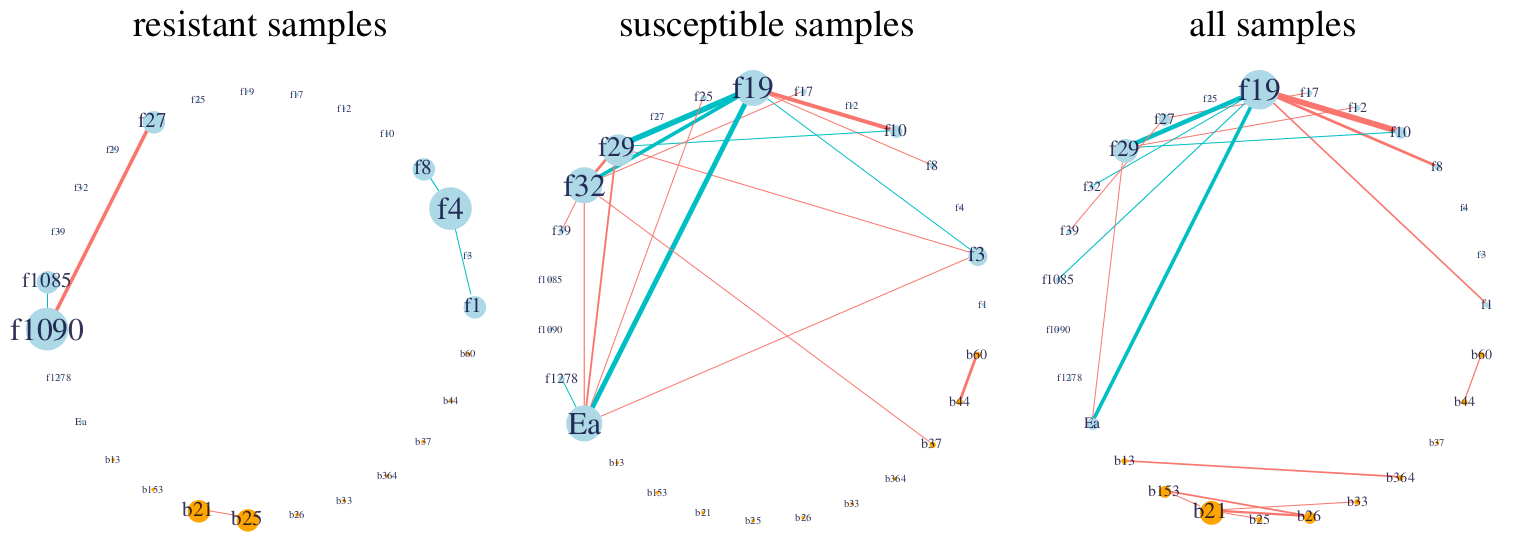
\includegraphics[width=.8\textwidth]{\fignet/CMR19-ICML-Fig3a}
  $$

}

%==================================================================
\frame{\frametitle{Oak mildew (2/2)}

  \begin{tabular}{cc}
    \hspace{-.04\textwidth}
    \begin{tabular}{p{.45\textwidth}}   
      \paragraph{Model selection.} As $\lambda$ decreases:
      \begin{itemize}
       \item the log-likelihood increases
       \item the number of parameters increases
      \end{itemize}
      
      \bigskip \bigskip 
      \paragraph{Penalized likelihood} criterion
      \begin{itemize}
       \item BIC
       \item EBIC
      \end{itemize}      
            
      \bigskip \bigskip 
      \paragraph{Robustness assessment} via resampling.

    \end{tabular}
    &
    \hspace{-.05\textwidth}
    \begin{tabular}{p{.45\textwidth}}   
      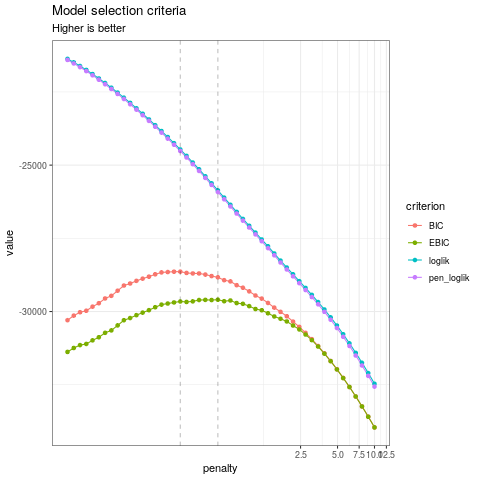
\includegraphics[width=.5\textwidth]{\fignet/JC2BIM-OaksPLN-netSel-full}
    \end{tabular}
  \end{tabular}


}
